%%
%% Beuth Hochschule für Technik --  
%%
%% Kapitel 3 -
%%
%%	


%%%%%%%%%%%%%%%%%%%%%%%%%%
%% bild einfügen:

%\begin{figure}[h]
%	\begin{center}
%		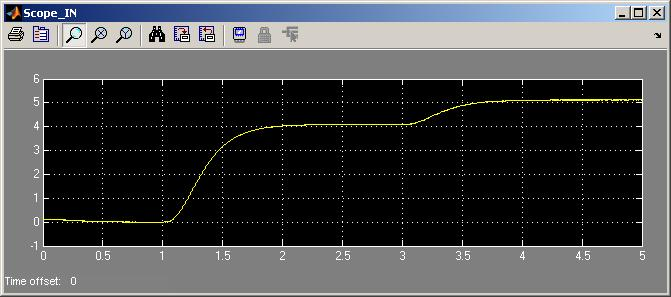
\includegraphics[scale=0.5]{sprungantwort.jpg}
%		\caption{bildbeschreibung - titel}
%       \label{für referenzen}
%	\end{center} 
%\end{figure}


%wenn du auf das bild refenzieren willst schreibst du \ref{...} wo ... = der inhalt von \label{•}

% sys_id = sys\_id ...... für latex _ = \_

%namen von dateien und tools bitte immer italic --> \textit{.....}

% mathematische werte zB 0,5V schreibst du so: $0,5V$

\newpage
[Perkowski]
\section{Messtechnische Identifikation des Steuerverhaltens der Strecke}\label{Kapitel3}


\subsection{Dynamisches Verhalten}

Zur Ermittlung des dynamischen Verhaltens wird eine Messung durchgeführt, in der das System zum Arbeitspunkt ($4V$) gebracht wird. Wenn das System einen stationären Zustand erreicht hat, wird erneut ein Sprung ($1V$) auf das System gegeben.

\begin{figure}[h]
	\begin{center}
		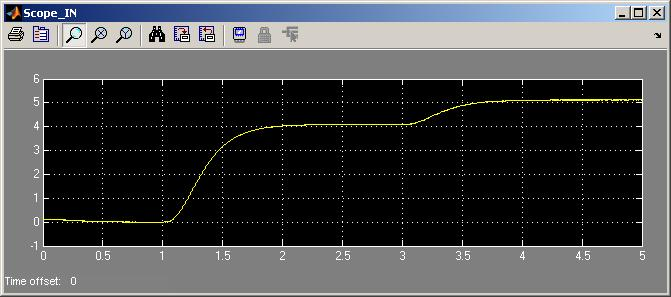
\includegraphics[scale=0.5]{sprungantwort.jpg}
		\caption{Sprungantwort - dynamische Kennlinie}
       \label{dynsprant}
	\end{center} 
\end{figure}

Wie in der Abbildung \ref{dynsprant} zu erkennen ist, bleibt die Verstärkung des Systems im Arbeitspunkt gleich.

\subsection{Identifikation der Strecke}
Mit Hilfe des Tools \textit{sys\_id.m} können wir die Strecke identifizieren. Dafür müssen die Vektoren \textit{ySystem} (Sprungantwort), \textit{uerr} (Sprung) und \textit{t} (Zeitachse) im Workspace bekannt sein. Im Tool \textit{sys\_id.m} muss eine Vorauswahl der Übertragungsglieder erfolgen. Da die Sprungantwort am Anfang eine Verzögerung hat, handelt es sich mindestens um ein PT2-Glied. Nach der Ausführung von \textit{sys\_id.m} ist in der Benutzeroberfläche (Abbildung \ref{pic_sis_id}) zu sehen, dass die Strecke aus einem System besteht, welches aus in Reihe geschalteten PT1, PT2 und PT3 Gleidern besteht. Die Parameter der Übertragungsfunktion in V-Normalform können abgelesen werden. 
Mit dem Button \textit{"Model speichern"} kann die Übertragungsfunktion als \textit{.mat} Datei im Workspace abgespeichert werden.

\newpage

\begin{figure}[h]
	\begin{center}
		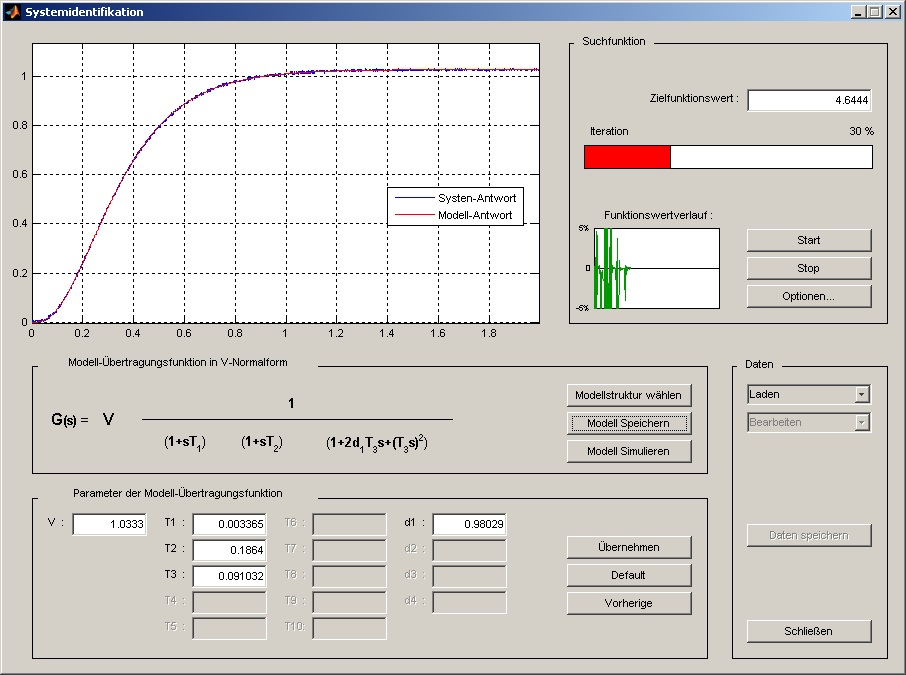
\includegraphics[scale=0.5]{sysid.jpg}
		\caption{Tool \textit{sis\_id} für Identifikation der Strecke}
       \label{pic_sis_id}
	\end{center} 
\end{figure}

Die ermittelte Übertragungsfunktion aus dem Tool \textit{sis\_id}: 

\begin{center}
$ G(s) = \dfrac{1,03}{(1 + 0,003365s) * (1 + 0,1864s) * (1 + 2*0,98029s + (0,091032s)^{2}) }$
\end{center}

Ausmultiplizierte Übertragungsfunktion für Polkompensation:

\begin{center}
$ G(s) =  \dfrac{1,03}{0,000005s^{4} + 0,0017s^{3	} + 0,043s^{2} + 0,368s + 1 } $
\end{center}
